\documentclass[a4paper,10pt]{article}
%\documentclass[a4paper,10pt]{scrartcl}
\usepackage{graphicx}
\usepackage[utf8]{inputenc}
\usepackage{listings}
\usepackage{hyperref}
\usepackage{indentfirst}
\usepackage{float}

\title{
Rapport de développement d'applications Web\\
Projet 2022 : Création d'un site de formation
}
\author{
Bertoux Hugo, Hamidou Nazim, Verstracte Valentin\\
Petit Evan, Perion Maxence, Pinon Alexandre
}
\date{}

\renewcommand*\contentsname{Sommaire}
\renewcommand{\listfigurename}{Liste des images}%

\begin{document}

\maketitle 
\tableofcontents

\newpage
\section{Introduction}
L'objectif de ce projet a été de réaliser un site de formation destiné à des apprenants/étudiants. Nous avons basé la construction de notre site autour d'un jeu vidéo nommé ``League Of Legends" et c'est pour cette raison que nous avons décidé de l'appeler ``E-lolning". Il se calque sur le fonctionnement de plusieurs sites de coaching en esport comme https://www.skill-capped.com/lol/.
Dans ce rapport, nous allons aborder tous les aspects de la conception de notre site, c'est-à-dire que nous allons aussi bien expliquer la modélisation, le modèle MVC utilisé et tout ce qui peut-être fait sur notre site. Il est important de rappeler qu'un site de formation en ligne ou site d'e-learning dans notre cas pour un jeu vidéo, permet aux utilisateurs de celui-ci de développer leurs compétences en participant à différents cours et discuter à propos de ce même cours dans un forum entre apprenants. Dans notre cas, nous donnons également la possibilité de créer un cours à qui le souhaite afin de partager son savoir et ses connaissances. 

\section{La gestion du projet}
Qui a fait quoi ? Comment on a repartie les taches ? Reunion ? Trello qui a permis d'organiser l'ensemble, méthodes scrum...

\section{La modélisation}
La problématique de la modélisation s'est centrée autour de deux points : Le diagramme use-case afin de pouvoir discerner toutes les fonctionnalités à implémenter, ainsi que le diagramme relationnel afin de s'assurer d'avoir un schéma de données correctement normalisé et logique avant même d'y stocker des données.\\
Nous pensons que l'étape du diagramme de classe n'est pas nécessaire puisque nous n'utilisons pas la programmation objet.

\subsection{Diagramme Use-Case}
\centerline{
    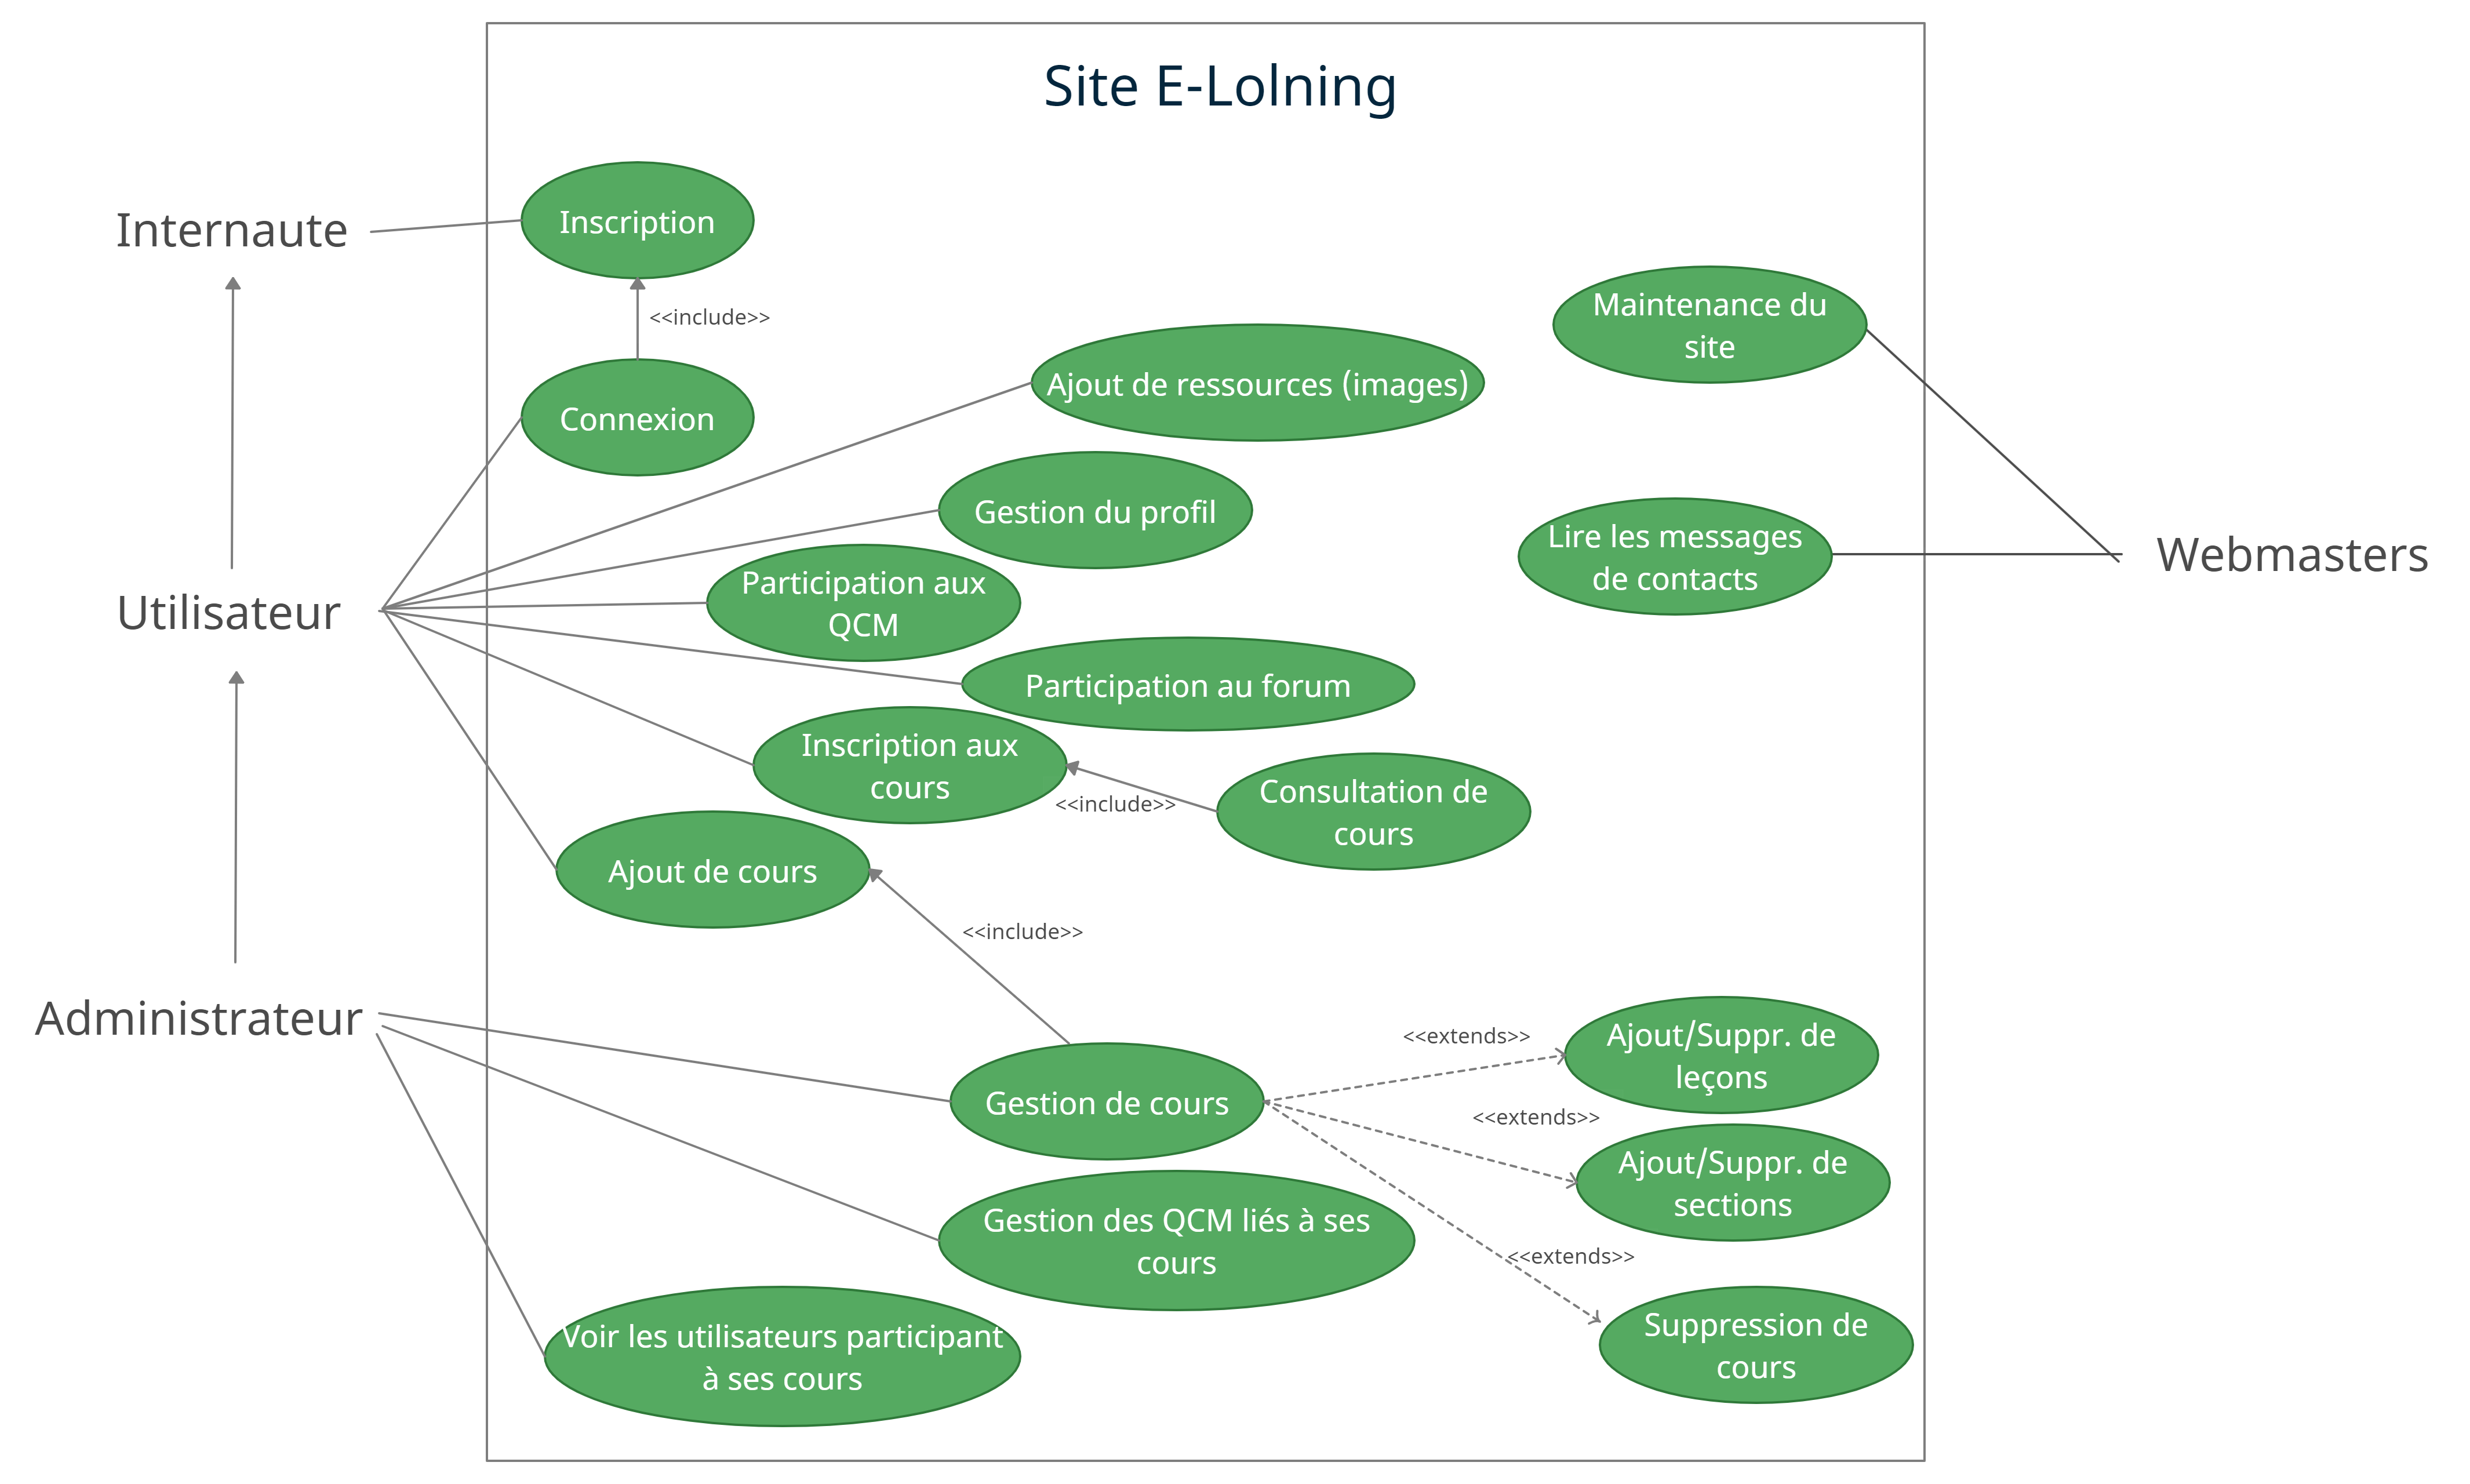
\includegraphics[width=19cm]{images/UseCase.png}
}
Nous considérons le besoin de spécifier 4 acteurs chez les utilisateurs de notre site, qui correspondent à leurs "droits". Cela est fait avec la notion spécification/généralisation d'acteurs :\\\\

\textbf{L'internaute :} Il s'agit d'un simple visiteur du site. L'internaute n'a pas accès aux cours, mais seulement à la page d'accueil et la possibilité de s'inscrire.\\\\

\textbf{L'utilisateur :} Correspond aux \textbf{Apprenants} dans l'énoncé du sujet. L'utilisateur est un internaute qui s'est connecté. Il est bon de noter que la connexion n'est possible qu'après l'inscription, ce qui fait apparaître la notion de $<<include>>$ de UML. Nous considérons qu'un utilisateur a accès à tous les cours du site, et il peut créer les siens : Dans ce cas il devient l'Administrateur de son propre cours (voir plus bas).
L'utilisateur a accès à un panneau d'administration qui lui permet de gérer son profil, ajouter des cours, et aussi ajouter des ressources liées à son compte : Ce sont des images qu'il peut utiliser dans ses cours, et qui sont hébergées dans notre base de donnée (via des BLOBs). Enfin, il peut participer au forum (créer des topics, répondre à ceux des autres utilisateurs, etc...).
Pour consulter un cours, un utilisateur doit s'y être inscrit. Cela permet à l'administrateur de savoir si son cours a du succès ou non.\\\\

\textbf{L'administrateur :} Correspond au titre du même nom dans l'énoncé du sujet. Il s'agit du statut d'un utilisateur dans son propre cours. Il peut rajouter des leçons, les supprimer, gérer ses QCM, etc... :  Afin de modéliser ces choix liés à la gestion d'un cours, encore une fois, nous pouvons profiter d'une notion d'UML. Cette fois-ci des $<<extends>>$ \\\\

\textbf{Les Webmasters :} Un comité très réduit d'utilisateurs possédant tous les droits sur le site. Ils ont un accès total au code source, à la base de données, et ont accès à une page leur permettant de voir des messages que les utilisateur leur ont envoyé via un formulaire de contact.
\newpage
\subsection{Diagramme Relationnel (et base de données)}

Les données sont stockées sur une base de données MySQL dont voici le schéma relationnel : \\\\

\centerline{
    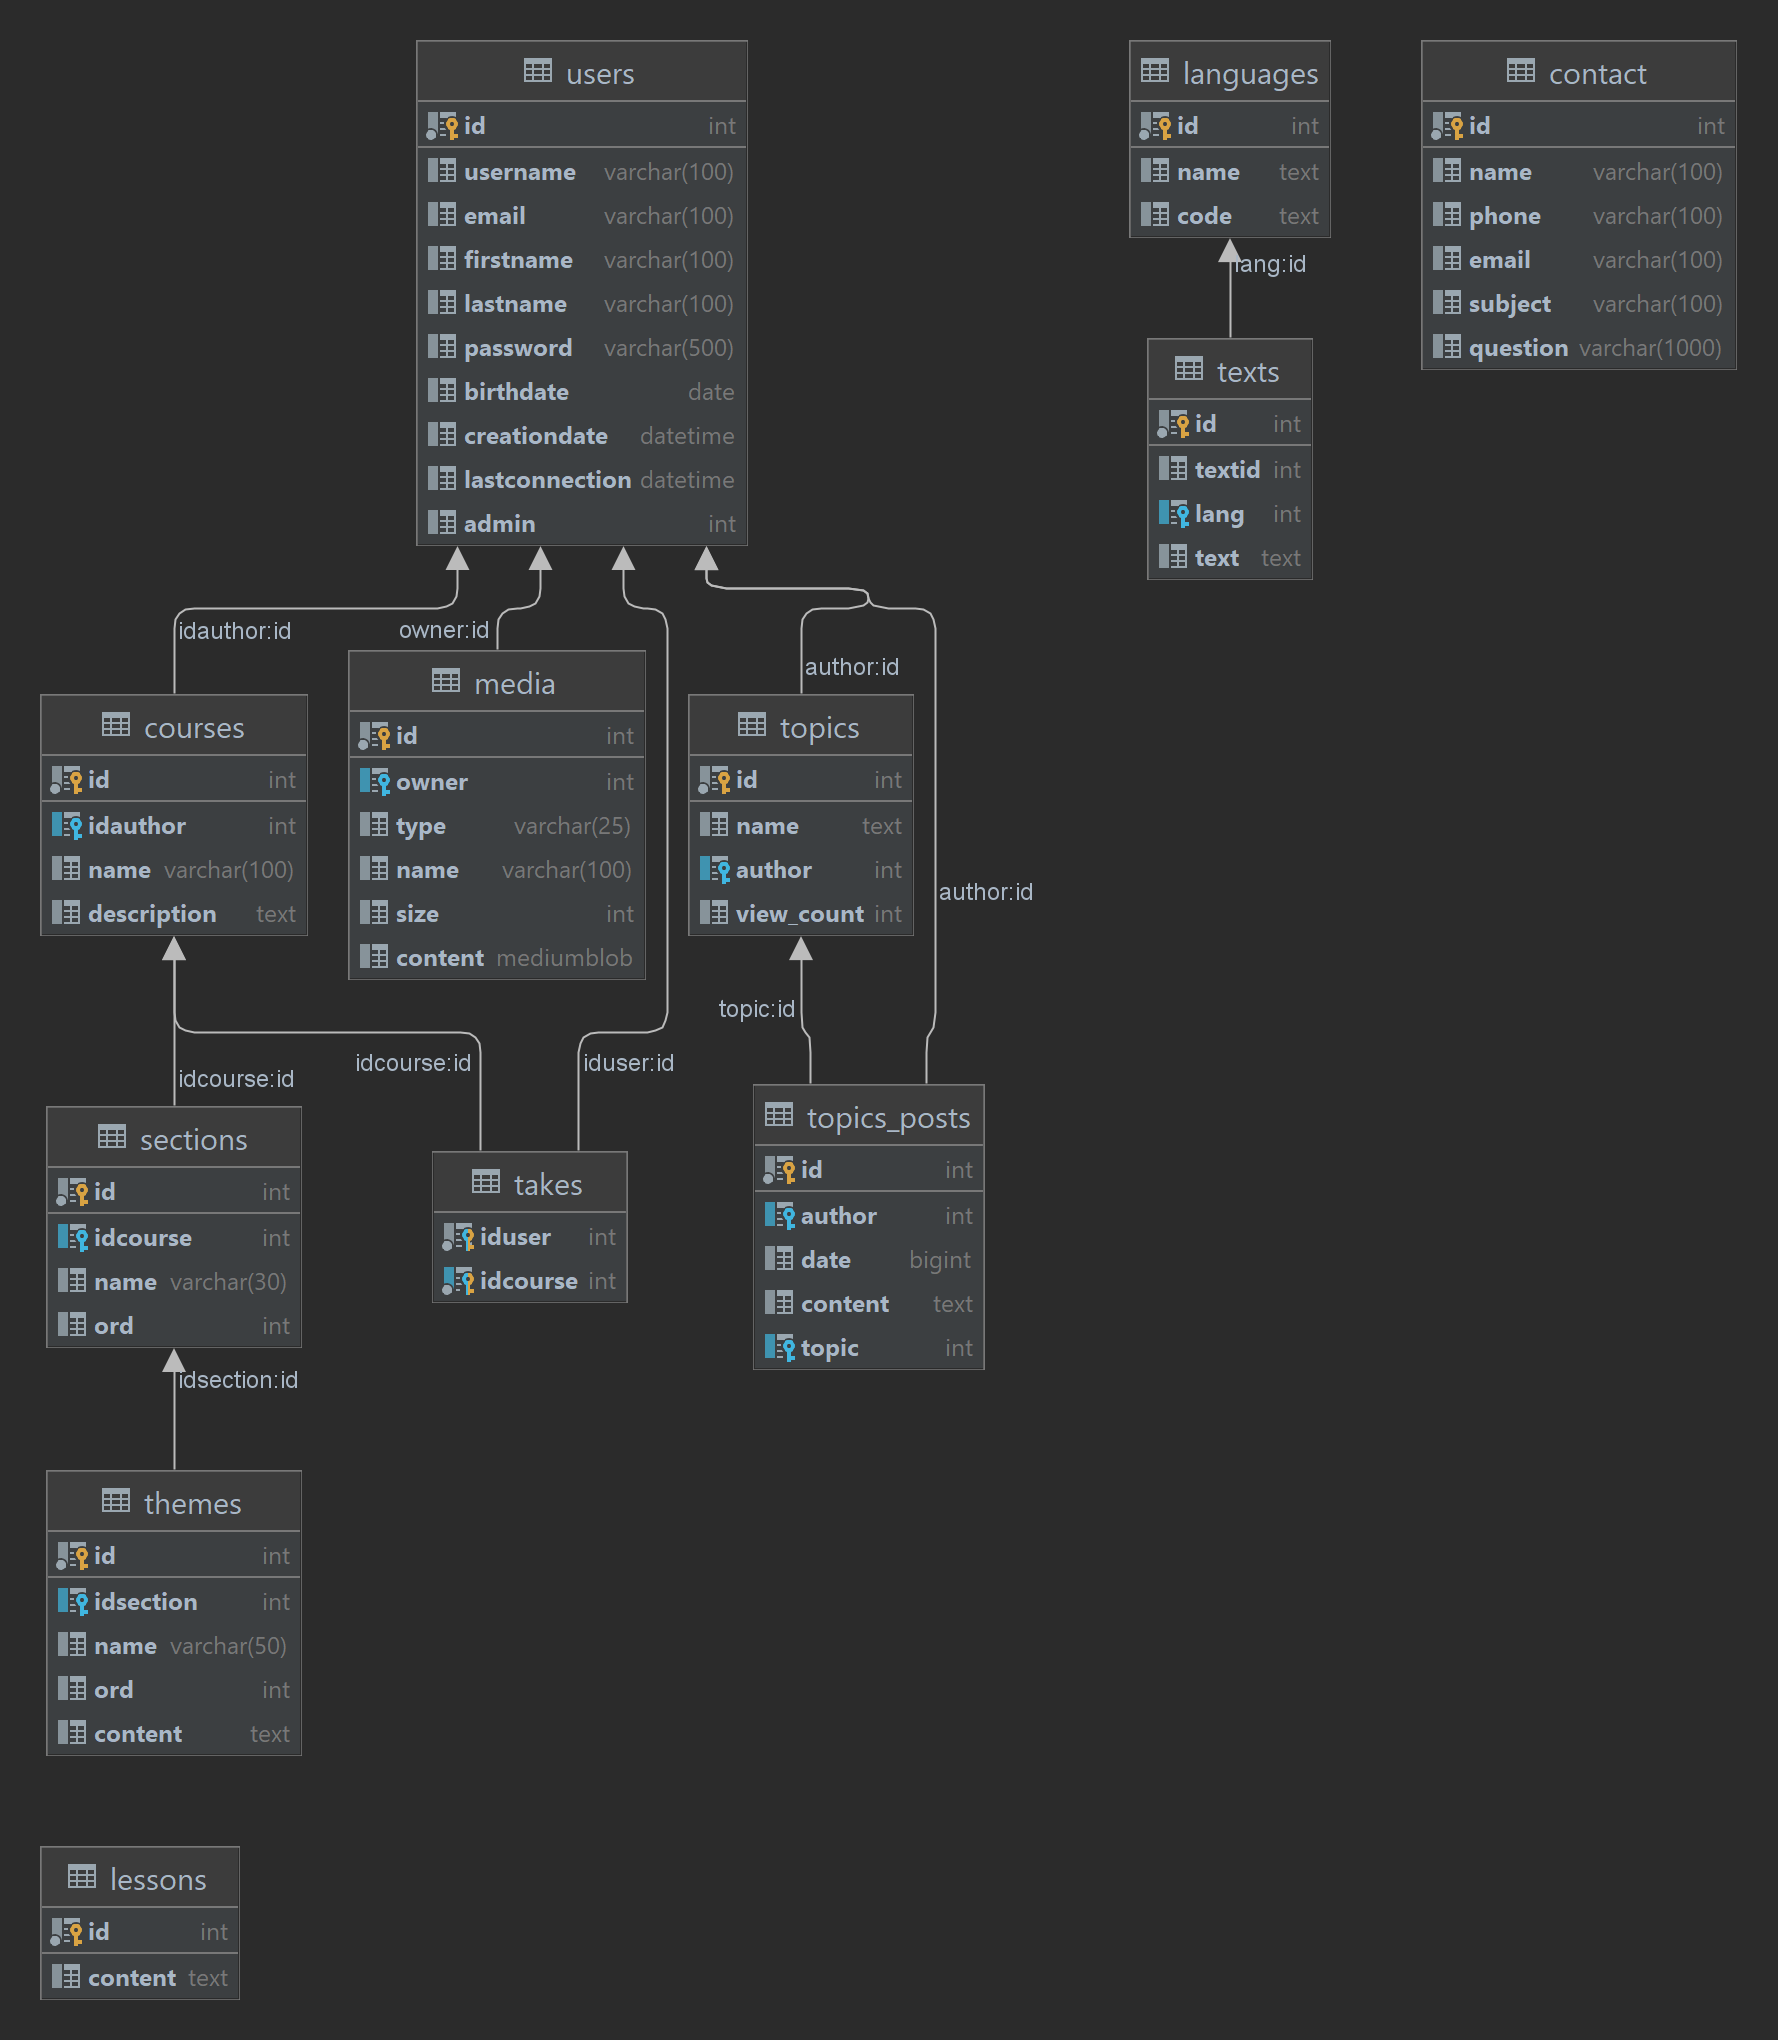
\includegraphics[width=16cm]{images/DB.png}
}
Nous ne montrons que les tables liées à la modélisation du site, puisqu'une multitude d'autres tables sont nécessaire à l'administration de la base de donnée, crée ou non par MySQL.\\\\
Les images sont stockées directement dans la base de donnée au format MediumBlob (voir table media)\\\\
La table est faite de sorte à ce que la suppression d'un utilisateur supprime en cascade toutes entrées dans la table lui étant liées, comme ses cours, ses topics, etc...\\\\
Voici un cours descriptif de chaque table. Premièrement, toutes les tables liées aux utilisateurs :
\begin{itemize}
\item[\textbf{users}] Stocke toutes les informations liées à un utilisateur à son inscription. Le boolean "admin" est mis à true s'il s'agit d'un webmaster.
\item[\textbf{courses}] Répertoire de tous les cours du site. Ils sont liés par clé étrangère aux utilisateurs les ayant crées.
\item[\textbf{sections}] Répertoire de chaque section (chapitres) de chaques cours. Ils sont liés par clé étrangère aux utilisateurs cours dont ils sont les chapitres
\item[\textbf{themes}] Répertoire de chaque leçon de chaque section. Ils sont liés par clé étrangère aux sections dont ils sont les leçons.
\item[\textbf{takes}] Associe un utilisateur a un cours, et signifie que l'utilisateur est inscrit à ce cours.
\item[\textbf{topics}] Stocke les topics do forum. Un topic est un fil de discussion basique, auquel chaque utilisateur peut répondre. Il est lié par clé étrangère à l'utilisateur qui l'a crée.
\item[\textbf{topics-posts}] Stocke les messages postés sur les topics. Liés par clé étrangère aux topics dont ils sont les réponses, et aux utilisateurs les ayant postés.
\end{itemize}

Il existe aussi un groupe de deux tables permettant la traduction en anglais et en français des contenus du site : 

\begin{itemize}
\item[\textbf{languages}] Liste les langages disponibles sur notre site
\item[\textbf{texts}] Table permettant d'inscrire la traduction d'un même texte en français et en anglais
\end{itemize}

Enfin, deux tables solitaires :

\begin{itemize}
\item[\textbf{contact}] Liste tous les messages adressés aux créateurs du site via le formulaire de contact.
\item[\textbf{lessons}] Version obsolète de la table themes
\end{itemize}
\newpage

\section{Notre installation}
Pour l'installation nous avons utilisé un serveur LAMP. Celui-ci tourne sous une VM avec Debian 11, 8 GO de RAM et 4 cœurs. Cette même VM est contenu dans un hyperviseur de type 1 qui est installé dans un HP DL380P G8 physiquement présent chez l'un de nos développeurs. \\
Un tel choix a été fait pour ajouter des plus valus qui aurait été indisponible avec une installation à l'université. Nous avons un contrôle total et nous avons par exemple notre propre adresse web : https://daw.privatedns.org/ 
Sur cet VM nous avons également installé MySQL, un outil que nous maitrisons et connaissons. \\ 
Pour gérer notre code nous utilisons github. Une "pipeline" a été mise en place pour déployer automatiquement le code source sur le serveur LAMP.

\section{La charte graphique}
Une charte graphique a été établie, comportant police d'écritures, tailles de police, couleurs pour le CSS, etc...
Les couleurs ont étées choisies à l'aide de : https://coolors.co/

\section{L'architecture MVC}
\subsection{Modèle}
Dans notre projet, les Contrôleurs appellent les Modèles pour deux raisons: Aller chercher des données dans la base de donnée dans la plupart des cas, ou bien les fichiers XML stockés sur notre serveur.\\
Dans ces deux cas, nous utilisons les fonctions natives à PHP qui permettent de dialoguer avec la base de données MySQL et de modifier, créer ou supprimer des fichiers sur le serveur.
\subsection{Vue}
Les vues permettent l'affichage des pages HTML au client grâce à php. Ce sont des fichiers PHP qui vérifient les droits de l'utilisateur courant grâce aux différents cookies, et sessions (est-ce un administrateur? est-il connecté?), et appelle diverses fonctions vis-à-vis de ces droits pour afficher certains éléments de la page : \\
Un utilisateur connecté n'a pas besoin de voir le bouton "se connecter", un élève ne doit pas avoir accès au bouton "modifier le cours" ou "ajouter une leçon".\\ \\
Lorsque certaines données ont besoin d'être récupérées, par exemple pour afficher le contenu d'un cours, le pseudo de tous les utilisateurs, etc... Un appel est fait au contrôleur correspondant.
\subsection{Contrôleur}
Les contrôleurs sont des fichiers PHP qui permettent de faire appel aux modèles via les vues. Les données récupérées sont souvent brutes (les tables clé-valeur qui sont retournées par MySQL par exemple)\\\\
Avec les contrôleurs, nous nous assurons que les données récupérées sont traitées et affichables à l'utilisateur afin que la vue puisse l'afficher correctement.

\newpage
\section{L'inscription/Connexion}
Le principe ici est assez simple et s'inspire de tout site web moderne.Des expressions régulières ont été ajoutées pour pouvoir contrôler les entrées, du genre le nom et prénom ne doivent pas contenir autre chose que des lettres, le nom d'utilisateur ne doit contenir que des lettres et des chiffres.Un contrôle de présence de chacune des entrées à été mis en place (on peut pas s'inscrire sans email par exemple).

Chaque erreur (si présente) est directement transmise à l'utilisateur pour qu'il puisse la corriger avant de pouvoir valider son inscription.

\section{Les cours}
\subsection{Quizz}
Les quiz vont être proposés pour les apprenants. Les quiz doivent être sous le format XML, on va donc partir sur un document XML par cours .Celui-ci sera créer a la création du cours.
Voici la DTD de notre quiz : 
\begin{lstlisting}[language=XML]
  <?xml version="1.0" encoding="UTF-8"?>
  <!ELEMENT Questionnaire (question+)>
  <!ATTLIST Questionnaire chapitre NMTOKEN #REQUIRED>
  <!ATTLIST Questionnaire Nom CDATA #REQUIRED>
  <!ELEMENT question (difficulte,intitule,choix+,reponse+)>
  <!ATTLIST question id NMTOKEN #REQUIRED>
  <!ELEMENT difficulte (#PCDATA)>
  <!ELEMENT intitule (#PCDATA)>
  <!ELEMENT choix (#PCDATA)>
  <!ATTLIST choix id NMTOKEN #REQUIRED>
  <!ELEMENT reponse (#PCDATA)>
\end{lstlisting}
On peut donc voir qu'une question aura un id associé, une difficulté, son intitulé ainsi que 4 choix et sa réponse.
Et donc lors de la création du cours, un document XML de cette forme sera créer : 
\begin{lstlisting}[language=XML]
  <?xml version="1.0" encoding="UTF-8"?>
  <!DOCTYPE Questionnaire SYSTEM "quiz.dtd">
  <Questionnaire chapitre="idducours" Nom="nomducours"> 
  </Questionnaire>
\end{lstlisting} 

Ainsi l'administrateur de son cours pourra par la suite venir ajouter ou supprimer des questions de son cours. 

Du côté des apprenants, ils pourront passer le quiz dans le cours associé. La liste des questions s'affichera et ils pourront y répondre en cliquant sur le choix qui veulent faire et ensuite valider le questionnaire.
A la fin , ils verront leurs notes et pourront repasser le test s'ils ont envie de faire mieux.
\subsection{Forum}
Le forum permet la discussion entre apprenants. Il est global et les utilisateurs peuvent créer un nouveau sujet ou répondre dans un déjà créé s'ils sont connectés. Ils peuvent également consulter la liste des sujets et les messages dans ceux-ci. Les utilisateurs connectés ont également la possibilité de modifier ou supprimer les sujets et les messages dont ils sont les auteurs. 


\section{Les options}
\subsection{Multilingue}
La première option que nous avons implémentée est un support multilingue ou plurilingue. Les différentes langues implémentées sont le Français et l'Anglais pour tous les utilisateurs. Nous avons fait cet ajout dans un soucis d'utilisation étrangère de notre site. En effet, nous nous sommes basés sur un jeu de renommée mondiale avec plusieurs milliers de millions d'utilisateurs annuels, et forcément parmi tous ces utilisateurs tous ne parlent pas couramment Français.\\

Afin de changer la langue il suffit de cliquer sur ce menu déroulant:
\begin{figure}[!h]
\centerline{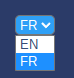
\includegraphics[width=4cm]{images/menuLangues.PNG}}
\caption{Les différentes langues proposées.}
\label{fig}
\end{figure}

Pour ce qui est de la partie technique, nous avons dans notre base de données la table ``texts" où sont inscrit tous les textes à afficher selon un identifiant de texte (qui est le même peu importe la langue) et une langue. Ensuite, il nous suffit d'afficher la traduction souhaitée dans le site après avoir récupéré la langue renseignée par l'utilisateur. Seules les traductions pour la langue anglaise et française sont actuellement disponibles, cependant le système a été conçu de façon scalable, c'est à dire que l'ajout d'une nouvelle langue dans la base de données rendra directement disponible cette langue pour les utilisateurs, sans que nous aillons à modifier quoi que ce soit dans nos scripts php. Cela est rendu possible grâce à une table ``languages" qui renseigne les différentes langues (abréviation, code, clé, ...) et la sélection de la langue depuis le site lit ces informations pour les afficher dans le sélecteur. La langue pour chaque traduction dans la table  ``texts" est une référence (clé étrangère) sur la clé de la table ``languages".

\subsection{Thèmes}
Notre site d'e-learning possède une option qui permet de changer de thèmes, c'est-à-dire passer du thème clair (thème par défaut) au thème sombre. Les différents thèmes sont utilisables par tous les utilisateurs à leur bon vouloir. L'intérêt d'utiliser des thèmes sont les suivants: le thème sombre permet de réduire la fatigue des yeux et les différents thèmes sont plus approprié à certaines conditions par exemple en pleine nuit le thème sombre sera plus apprécié.\\

Les utilisateurs peuvent changer de thèmes par l'intermédiaire de ce bouton:
\begin{figure}[!h]
\centerline{
    
\includegraphics[width=4cm]{images/boutonThemeClaire.PNG}
    
\includegraphics[width=4cm]{images/boutonThemeSombre.PNG}
}
\caption{Bouton en mode thème clair.}
\caption{Bouton en mode thème sombre.}
\label{fig}
\end{figure}

Le fonctionnement des thèmes est assez simple, en effet il nous suffit de déclarer 2 fichiers css que nous avons nommés respectivement ``lightMode.css" et ``darkMode.css". Dans ces fichiers sont déclarées des variables avec ``--nomVariable" correspondant aux couleurs qui seront utilisées dans leurs thèmes respectifs. Pour ces deux fichiers les variables doivent avoir le même nom mais avoir évidemment des valeurs différentes. Une fois ceci effectué, nous allons utiliser seulement les variables contenus dans les fichiers ``lightMode.css" ou ``darkMode.css" via différentes fonctions jQuery créés par nos propres moyens permettant d'importer un fichier ou un autre selon le thème. Les feuilles de styles vont ensuite définir, pour chaque page, le style à appliquer en utilisant des variables à la place des couleurs grâce à la syntaxe ``var(--nomVariable)". Finalement pour avoir un thème permanent et ne pas avoir besoin de repasser dans le thème souhaité à chaque rafraîchissement ou changement de page, nous avons utilisé un cookie. Ce cookie permet de stocker la valeur du thème choisi et avec le traitement de nos fonctions en jQuery, charger le bon thème.\\

Pour illustrer ce qui a précédemment été vu, voyons avec un exemple concret. Nous définissons une variable ``--background-color: \#FFFFFF;" pour le thème clair et ``--background-color: \#000000;" pour le thème sombre. Maintenant dans un fichier css quelconque on peut utiliser ceci:
\begin{lstlisting}[language=HTML]
  body{
    background-color: var(--background-color);
  }
\end{lstlisting}
Si le thème clair est utilisé alors la couleur de fond aura pour valeur FFFFFF c'est-à-dire blanc, et dans le cas contraire pour le thème sombre la couleur de fond aura pour valeur 000000 c'est-à-dire noir.

\subsection{Décompte des visiteurs}
Dans une dynamique de création d'options agréables pour tous, nous avons intégré un compteur du nombre de visiteur, ce compteur est affiché dès l'arrivée de l'utilisateur sur la page d'accueil. Afin de stocker le nombre de visiteur de notre site nous l'avons fait via un fichier et non base de données car PHP permet la gestion de ce genre de petit fichier. Le fichier se nomme tout simplement "compteur.txt" et contient le nombre de visiteurs.\\

Voici un aperçu de l'affichage en question: 
\begin{figure}[!h]
\centerline{
\includegraphics[width=8cm]{images/numberVisiteurs.PNG}}
\caption{L'affichage du nombre de visiteur.}
\label{fig}
\end{figure}

\subsection{Contacter le support du site}
Finalement, pour tous utilisateurs ayant la moindre question que ce soit sur le site, un cours en particulier ou d'autres informations, alors l'utilisateur peut nous faire parvenir un message via la section ``Contact" sur la page d'accueil. Pour envoyer à sa requête, il faut remplir les champs nécessaires sur cette page. Si le message est correctement traité alors un message de confirmation d'envoi est affiché. L'utilisateur peut ensuite attendre une réponse via l'un des moyens de contact qu'il a renseigné. Pour l'équipe d'administration, il existe une catégorie supplémentaire dans la partie profil. Cette catégorie se nomme ``Manage contacts" et elle permet d'afficher l'ensemble des messages envoyés par les utilisateurs. Ces messages peuvent être supprimés par les Webmasters, mais ils sont également dans la possibilité de répondre à ces messages via un ``mailto''.\\

Voici à quoi ressemble la page de gestion des messages:
\begin{figure}[!h]
\centerline{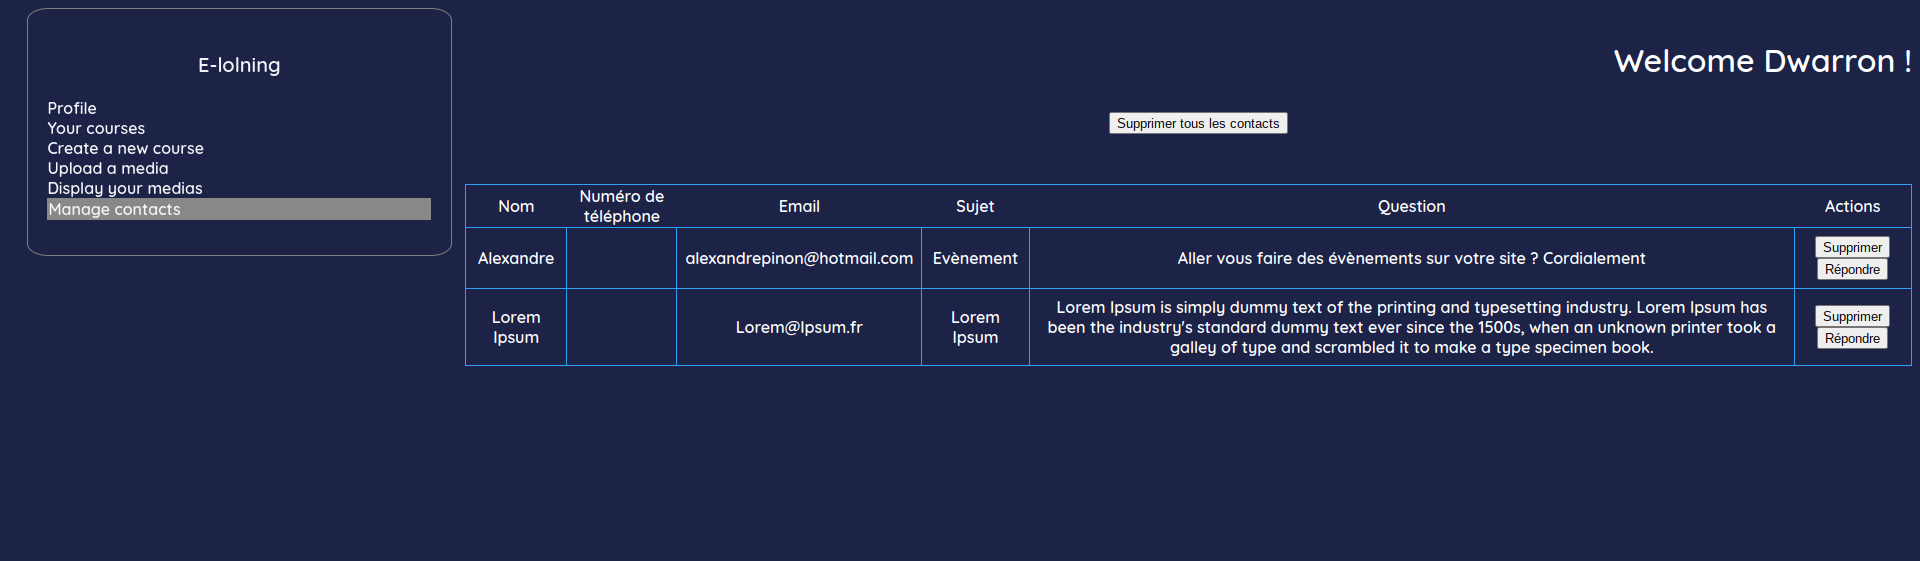
\includegraphics[width=16cm]{images/manageContact.PNG}}
\caption{L'affichage des messages pour les Webmasters.}
\label{fig}
\end{figure}

Dernièrement, les messages sont stockés dans la table ``contact" de la base de données et les administrateurs sont définis par un booléen dans la table ``users" que nous pouvons ajouter à la main.

\section{Conclusion}


\end{document}
